\chapter{Problemi NP-completi} \label{ch:capitolo13}
\subsection{3SAT}
\textbf{Proposizione}\\
Il problema 3SAT è NP-completo.\\\\
\textbf{Dimostrazione}      
\begin{itemize}
    \item Chiaramente 3SAT $\in$ NP.
    
    \item Per provare che 3SAT è NP-arduo, basta SAT $<=_p$ 3SAT.
    
    \item Dobbiamo associare a ogni sistema di clausole un sistema di 3-clausole, calcolabile in tempo polinomiale, preservando soddisfacibilità e insoddisfacibilità.
\end{itemize}
\textbf{Esempio}\\
Se sostituisco la clausola $x_1, \Bar{x}_2, x_3, x_4$ con le due clausole
\begin{center}
    $x_1, \Bar{x}_2z_1, \Bar{z}x_3x_4$
\end{center}
ove z è una nuova variabile, la (in)soddisfacibilità è preservata.
\begin{itemize}
    \item Si può usare la medesima tecnica per tutte le clausole di lunghezza $>=$ 4.
\end{itemize}
\textbf{Esempio}\\
Se sostituisco la clausola $x_1, \Bar{x}_2$ con le due clausole
\begin{center}
    $x_1, \Bar{x}_2y, x_1, \Bar{x}_2\Bar{y}$
\end{center}
ove y è una nuova variabile, la (in)soddisfacibilità è preservata.
\begin{itemize}
    \item Si può usare la medesima tecnica per tutte le clausole di lunghezza 2 e anche di lunghezza 1.
\end{itemize}
\textbf{Conclusione}\\
Con le regole precedenti si ottiene una riduzione di SAT a 3SAT. È facile convincersi che e la riduzione si calcola in tempo polinomiale.
Quindi SAT $<=_p$ 3SAT.
\subsection{Insieme indipendente}
\textbf{Proposizione}\\
Il problema IS è NP-completo\\\\
\textbf{Dimostrazione}
\begin{itemize}
    \item Si è già visto che IS $\in$ NP
    
    \item Per provare che IS è NP-arduo, basta 3SAT $<=_p$ IS.
    
    \item Dobbiamo associare a ogni sistema di 3-clausole S un grafo  G$_S$ e un intero m\_S , calcolabili in tempo polinomiale, tale che
    
    \begin{center}
        \begin{figure}[htp]
            \centering
            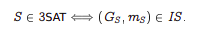
\includegraphics[scale=0.9]{tesi_stile/img/foto1cap13.png}
        \end{figure}
    \end{center}
\end{itemize}
\textbf{Esempio}\\
\begin{figure}[htp]
    \centering
    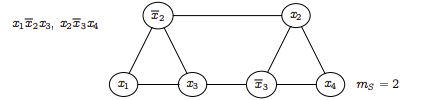
\includegraphics[scale=0.9]{tesi_stile/img/foto2cap13.png}
\end{figure}
\subsection{Ridurre 3SAT a IS}
\begin{itemize}
    \item 3 vertici per ogni clausola (corrispondenti ai 3 letterali)
    
    \item I lati connettono i 3 letterali di ogni clausola e ogni vertice con letterale x a tutti i vertici con letterale $\Bar{x}$
    
    \item m\_S = numero delle clausole
\end{itemize}
\textbf{Osservazione}\\
Un insieme di m\_S vertici indipendenti contiene esattamente un vertice di
ogni ‘triangolo’ e non contiene vertici etichettati con un letterale e il suo
opposto.\\\\
\textbf{Conclusione}\\
Con la costruzione precedente si ottiene una riduzione di 3SAT a IS.
È facile convincersi che la riduzione si calcola in tempo polinomiale.
Quindi SAT $<=_p$ 3SAT.
\subsection{CLIQUE e VC}
\textbf{Proposizione}\\
CLIQUE e VC sono NP-completi.\\\\
\textbf{Dimostrazione}\\
\begin{itemize}
    \item Si è già visto che questi due problemi sono in NP.
    
    \item Inoltre IS $<=_p$ VC e IS $<=_p$ CLIQUE
\end{itemize}
\subsection{3COL}
\textbf{Proposizione}\\
Il problema 3COL è NP-completo.\\\\
\textbf{Dimostrazione}\\
\begin{itemize}
    \item Si è già visto che 3COL $\in$ NP.
    
    \item Per provare che 3COL è NP-arduo, basta 3SAT $<=_p$ 3COL.
    
    \item Dobbiamo associare a ogni sistema di 3-clausole S un grafo  G$_S$ calcolabile in tempo polinomiale, tale che
    
   \begin{figure}[htp]
        \centering
        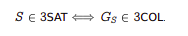
\includegraphics[scale=0.9]{tesi_stile/img/foto4cap13.png}
    \end{figure}
\end{itemize}
\subsection{Ridurre 3SAT a 3COL}
\begin{itemize}
    \item 3 vertici tutti collegati fra loro (chiamiamoli 0,1,2)
    
    \item Un vertice per ogni letterale, tutti collegati al vertice 2, inoltre ogni letterale collegato alla sua negazione
\end{itemize}
\begin{figure}[htp]
    \centering
    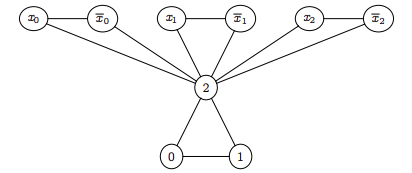
\includegraphics[scale=0.9]{tesi_stile/img/foto5cap13.png}
\end{figure}
\newpage
\subsection{Ridurre 3SAT a 3COL}
per ogni clausola $\lambda_1, \lambda_2, \lambda_3$, 5 nuovi vertici e le connessioni
\begin{figure}[htp]
    \centering
    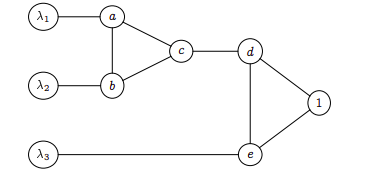
\includegraphics[scale=0.9]{tesi_stile/img/foto6cap13.png}
\end{figure}\\
\textbf{Osservazioni}\\
\begin{itemize}
    \item Assegnamo i colori 0,1,2 ai vertici 0,1,2
    
    \item I letterali avranno colore 0 o 1 e ognuno colore diverso dalla sua negazione
    
    \item Se \textit{e} ha colore 0, allora $\lambda_3$ = 1
    
    \item Se invece \textit{e} ha colore 2, allora, \textit{d} ha colore 0, una fra \textit{a} e \textit{b} ha colore 0, uno fra $\lambda_1, \lambda_2, \lambda_3$ ha colore 1.
    
    \item Quindi almeno uno tra $\lambda_1, \lambda_2, \lambda_3$ ha colore 1, si possono assegnare colori coerenti ai vertici, \textit{a, b, c, d, e}
\end{itemize}
\textbf{Conclusione}\\
Se G$_S$ ha una 3-colorazione, un letterale di ogni clausola ha colore 1: i letterali di colore 1 soddisfano S
Viceversa se S $\in$ 3SAT, G$_S$ ha una 3-colorazione coi letterali veri di colore 1 e i letterali falsi di colore 0.
\newpage
\subsection{Problemi NP-intermedi}
\textbf{Definizione}\\
Un problema è NP-intermedio se appartiene alla classe NP-P, ma non è
NP-completo.\\
Non è noto se esistano problemi NP-intermedi (potrebbero non esistere anche se P $\neq$ NP)\\\\
\textbf{Candidati}
\begin{itemize}
    \item Isomorfismi di grafi:
    
    \textbf{Input:} Due grafi G e G'\\
    \textbf{Output:} Si se esiste un isomorfismo tra G e G', NO altrimenti
    
    \item Decomposizione di un intero in fattori primi
    
    \item Problemi radi
    
    \item Problemi unari
\end{itemize}
\subsection{Problemi NP-intermedi}
\textbf{Definizione}\\
Un problema S è rado se il numero delle parole di S di lunghezza n è polinomialmente limitato.
Un problema S $\subseteq$ a* si dice unario.\\\\
\textbf{Proposizione}\\
Se esiste un problema rado in NP $-$ P, allora è necessariamente un problema NP-intermedio.\\\\
\textbf{Proposizione}\\
Se esiste un problema rado in NP $-$ P, allora ne esite uno unario.
\newpage
\subsection{Congettura di Berman-Hartmanis}
\textbf{Definizione}\\
Due problemi S, T su alfabeti A, B sono P-isomorfi se c’è una biiezione $f: A* \mapsto B*$ tale che
\begin{itemize}
    \item $f e f^-1$ sono computabili in tempo polinomiale
    
    \item per ogni $w \in A*$, si ha w $\in$ S $\Longleftrightarrow$ f(w) $\in$ T.
\end{itemize}
\textbf{Congettura}\\
Due problemi NP-completi sono sempre P-isomorfi.